\documentclass[tikz]{standalone}
% https://latexdraw.com/plot-a-function-and-data-in-latex/

\usepackage{tikz}
\usepackage{pgfplots}
%\usepackage{physics}
\pgfplotsset{compat = newest}
\begin{document}
    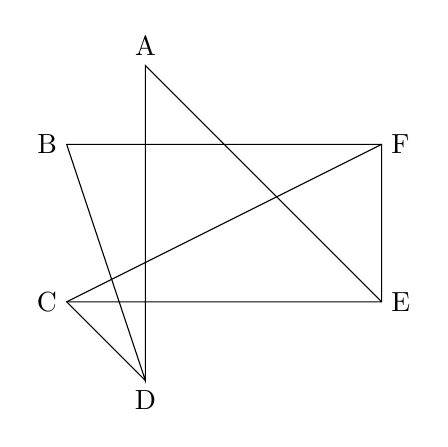
\begin{tikzpicture}
     \coordinate (A) at (1,3) node at (A) [above] {$\mathrm{A}$};
     \coordinate (B) at (0,2) node at (B) [left] {$\mathrm{B}$};
     \coordinate (C) at (0,0) node at (C) [left] {$\mathrm{C}$};
     \coordinate (D) at (1,-1) node at (D) [below] {$\mathrm{D}$};
     \coordinate (E) at (4,0) node at (E) [right] {$\mathrm{E}$};
     \coordinate (F) at (4,2) node at (F) [right] {$\mathrm{F}$};

     \draw(C)--(E)--(F)--(B)--(D)--(A)--(E);
     \draw(F)--(C)--(D);

    \end{tikzpicture}
\end{document}

% \documentclass{standalone}

% \usepackage{tikz}
% \usepackage{pgfplots}

% \pgfplotsset{compat = newest}

% \begin{document}
%     \begin{tikzpicture}
%         \begin{axis}[
%             xmin = 0, xmax = 30,
%             ymin = -1.5, ymax = 2.0,
%             xtick distance = 2.5,
%             ytick distance = 0.5,
%             grid = both,
%             minor tick num = 1,
%             major grid style = {lightgray},
%             minor grid style = {lightgray!25},
%             width = \textwidth,
%             height = 0.5\textwidth,
%             xlabel = {$x$},
%             ylabel = {$y$},
%             legend cell align = {left},
%         ]
%             \addplot[
%                 domain = 0:30,
%                 samples = 200,
%                 smooth,
%                 thick,
%                 blue,
%             ] {exp(-x/10)*( cos(deg(x)) + sin(deg(x))/10 )};
            
%             \addplot[
%                 smooth,
%                 thin,
%                 red,
%                 dashed
%             ] file[skip first] {cosine.dat};
            
%             \legend{Plot from expression, Plot from file}
%         \end{axis}
%     \end{tikzpicture}
% \end{document}